%\iffalse
%
%    \begin{macrocode}
%<*driver>
\documentclass{article}
\usepackage{doc}
\usepackage[american]{babel}
\usepackage[notoday]{rcsinfo}
\begin{document}
   \DocInput{ths.dtx}
\end{document}
%</driver>
%    \end{macrocode}
%\fi
%
% \rcsInfo $Id: ths.dtx,v 6.4 2015/02/17 19:12:42 khoman Exp $
% \title{Thesis/Dissertation Templates}
% \author{Kelly O.\ Homan, PhD\\
%         Associate Professor of Mechanical Engineering\\
%         Missouri University of Science \& Technology\\
%         Rolla, Missouri 65409-0050
%         \texttt{khoman@mst.edu}}
% \date{%
%    \LaTeX'd on \today\\
%    (Version~\rcsInfoRevision\ of\texttt{\rcsInfoFile} --- \rcsInfoLongDate)}
% \maketitle
%
% \begin{abstract}
%
% \end{abstract}
%
% \tableofcontents
%
% \section{Preface}
% 
% \subsection{File Description}
%
% Simply \LaTeX\ the \verb|ths.ins| file to generate the template
% files for a publication thesis option format thesis,
% \verb|ptotemplate.tex|, and a \LaTeX-standard report class thesis,
% \verb|rpctemplate.tex|, along with five variants of a thesis
% chapter. The variants include text only (\verb|chapmin.tex|), floats
% (\verb|chapflt.tex|), bibliography citations (\verb|chapbib|),
% nomenclature entries (\verb|chapglo.tex|), and all of the above
% (\verb|chapall.tex|).  The inclusion or removal of these various
% chapter templates allows one to verify a local \LaTeX\ installation
% and the associated compile stages.
%
% This documentation file (\verb|ths.dtx|) can
% be typeset by running it through \LaTeX.
% 
% \emph{Very important:} the \verb|<ps>| characters which appear in
% the code are simply a placeholder for a percent sign (\LaTeX\
% comment character).  These characters are used so that during the
% generation of the code output, these lines are not removed.  Bottom
% line, after \LaTeX'ing the \verb|ths.ins| file, do a replace all for
% \verb|<ps>| with \verb|%| to obtain a proper \LaTeX\ file.
%
% \subsection{Limitations and Bugs}
% 
% \begin{description} 
% \item [Added: 2014/10/21] The documentation text may not accurately
% reflect the current form of the code.  The code, however, is correct
% and produces properly functioning templates.
% \item [Added: 2011/10/24] 
%  The co-adviser specification does not work as indicated by the 
%  original template.  The command must have an error in it as the
%    command desires an argument, but when one is provided, it adds
%    the designation co-adviser to the committee memberone.
% \item [Resolved (Originally Added: 2011/11/03).] The first page of
%   each individual appendix in a thesis with multiple appendices is
%   not correctly generated in LaTeX.  At the moment, this would
%   require generating these pages outside of LaTeX.  The associated
%   class file will need revision in order to make these pages
%   generate with the correct formatting.
% \item [Added: 2008/01/23, Resolved: 2011/07/12]
%  At present the rpctemplate.tex will not be a function template.
%  This can be developed later on an as needed basis.  The intended
%  difference between the two templates is that the \verb|ptotemplate|
%  is a thesis based on the publication option whereas the
%  \verb|rpctemplate| is a thesis based on the report class and not
%  based on separately generated publication- formatted
%  manuscripts. 
% \end{description}
%
% \section{Hints for Final Edit Stage}
%
% The last stages of editing a thesis often come down to treating
%    widow and orphan lines.  The following are hints for addressing
%    these final issues:
% \begin{itemize}
% \item Use \verb|\enlargethispage{\baselineskip}| command.
% \item Add a \verb|\newpage| command to force the start of a new page
%    at a specific point.
% \item LaTeX has a parameter for 'penalty' for widows and orphans 
%    ('club lines' in LaTeX terminology). With the greater penalty
%    LaTeX will try more to avoid widows and orphans. You can try to 
%    increase these penalties by putting following commands in your 
%    document preamble:
%    \verb|\widowpenalty=300\clubpenalty=300|. If this does not help,
%    you can try increasing these values even more, to a maximum of 
%    10000. However, it is not recommended to set this value too high, 
%    as setting it to 10000 forbids LaTeX from doing this altogether, 
%    which might result in strange behavior.
% \item Although I have not tested this, Wikipedia suggests it also 
%    helps to have rubber band values for the space between paragraphs:
%    \verb|\setlength{\parskip}{3ex plus 2ex minus 2ex}|.
% \end{itemize}
%
% \section{\LaTeX\ Template for Standard Report Class Thesis}
%
% \subsection{Description}

% This template represents a thesis generated as a single report class
% document.
%
% I have used the \texttt{chapter} and \texttt{chapter*} commands to
% produce both chapter titles and titles for the frontmatter and
% backmatter.  In my opinion this is the easiest and most transparent
% method to produce absolutely uniform type and layout.  The thesis
% style files that I received tried to accomplish this using custom
% defined commands but the result was not satisfactory, in my opinion.
% The \texttt{chapter*} command produces no numbering, which is in
% fact true for any of the sectioning commands.
%
% One change which you, as a user, may wish to make is in the relative
% locations of the files.  For \LaTeX\, all relative file locations
% have to be given with respect to the file that will be compiled by
% \LaTeX. Thus, if it is desired to have chapter files in
% sub-directories of the directory containing the base \verb|*.tex|
% file, the include commands will need to be of a form such as
% \verb|\include{subdir/foo.tex}|. This same logic also applies to the
% locations used to specify the *.eps files in each of the chapter's
% \texttt{*.tex} files.  
% 
% The contents of \texttt{template.tex} are expected to be rather
% transparent.  The only thing that may be worth further explanation
% is the use of the \texttt{include} and \texttt{includeonly} commands
% instead of \texttt{input}.  The reason is that the
% include/includeonly combination allows one to conditionally load the
% files.  This can save time when only one chapter, or portion of the
% thesis, is begin worked on at a given time. The only danger to this
% approach is that if a given chapter is not part of the include only
% list, then its impact on pagination, lists of figures, tables, etc
% will be frozen.  A final run with all of the include files part of
% of the includeonly list will ensure a complete document.
%
% \subsection{Thesis Template}
%
% \subsubsection{Preamble}
%
%    \begin{macrocode}
%<*rpc>
 % -*- mode: LaTeX -*-
 % ... preamble ...
\documentclass[times,12pt,titlepage]{mstthesis}
\doublespacing
\usepackage{threeparttable}
\usepackage[final]{graphicx}
\usepackage{psfrag}
\usepackage[noprefix]{nomencl}
\makenomenclature
\renewcommand{\nomgroup}[1]{
   \ifthenelse{\equal{#1}{A}}{\medskip \item \textbf{Roman}}{}%
   \ifthenelse{\equal{#1}{G}}{\medskip \item \textbf{Greek}}{}%
   \ifthenelse{\equal{#1}{S}}{\medskip \item \textbf{Subscripts}}{}%
}
\usepackage[nopar]{lipsum} % ... provides dummy text ...

 % ... end preamble ...

\begin{document}

%    \end{macrocode}
%
% \subsubsection{Title Page}
%
%    \begin{macrocode}
 % ... specify: ms or phd ...

\begin{ThesisTitlePage}{ms}

 % ... title page info ...

\author{\MakeUppercase{I. M. Author}}

\thesistitle{\MakeUppercase{The Title of My Work}}

\department{Mechanical Engineering} 

 % ... thesis committee ...

\ThesisAdviser{Galileo}

 % If you have a co-advisor, enter the name in the 
 % curly braces below and uncomment.  
 % Otherwise, leave commented out.
 %\cothadviser{} % If you have 2 thesis advisers

\memberone{Newton}        
\membertwo{Copernicus}        
\memberthree{Laplace}
\memberfour{Fourier}
\memberfive{Prandtl}

 % ... Graduation date - NOT your submission date ...
\graddate{1685}       

\end{ThesisTitlePage}
%    \end{macrocode}
%
% \subsubsection{Copyright, Abstract, and Acknowledgments}
%
%    \begin{macrocode}
 % ... copyright page - true|false ...

\copyrightyear{1684}   
\ThesisCopyrightPage{true}

 % ... front matter - thesis abstract ...

\begin{ThesisAbstract}
\lipsum[1]
\end{ThesisAbstract}

 % ... front matter - thesis acknowledgements ...

\begin{ThesisAcknowledgment}
\lipsum[2]
\end{ThesisAcknowledgment}
%    \end{macrocode}
%
% \subsubsection{Contents, Illustrations, Tables and Symbols}
%
%    \begin{macrocode}
\begin{ThesisFrontMatter}
\tableofcontents 
\listoffigures 
\listoftables  
\listofsymbols
\end{ThesisFrontMatter}
%    \end{macrocode}
%
% \subsubsection{Thesis Body}
%
%    \begin{macrocode}

\begin{ThesisBody}

 % ... introduction chapter ...
\ThesisBodyChapter{Introduction}%%
%% This is file `chapmin.tex',
%% generated with the docstrip utility.
%%
%% The original source files were:
%%
%% ths.dtx  (with options: `chapmin')
%% 
%% IMPORTANT NOTICE:
%% 
%% For the copyright see the source file.
%% 
%% Any modified versions of this file must be renamed
%% with new filenames distinct from chapmin.tex.
%% 
%% For distribution of the original source see the terms
%% for copying and modification in the file ths.dtx.
%% 
%% This generated file may be distributed as long as the
%% original source files, as listed above, are part of the
%% same distribution. (The sources need not necessarily be
%% in the same archive or directory.)


 %% ... sample chapter ...

\lipsum[5]

\section{Introduction}
\lipsum[6-8]

\endinput
%%
%% End of file `chapmin.tex'.


 % ... conclusions chapter ...
\ThesisBodyChapter{Conclusions}%%
%% This is file `chapall.tex',
%% generated with the docstrip utility.
%%
%% The original source files were:
%%
%% ths.dtx  (with options: `chapmin,addfig,addtbl,addbib,addglo')
%% 
%% IMPORTANT NOTICE:
%% 
%% For the copyright see the source file.
%% 
%% Any modified versions of this file must be renamed
%% with new filenames distinct from chapall.tex.
%% 
%% For distribution of the original source see the terms
%% for copying and modification in the file ths.dtx.
%% 
%% This generated file may be distributed as long as the
%% original source files, as listed above, are part of the
%% same distribution. (The sources need not necessarily be
%% in the same archive or directory.)


 %% ... sample chapter ...

\lipsum[5]

\section{Introduction}
\lipsum[6-8]

\section{Section with Figures and Heading Which is Really Long So
That It Produces a Two-Line Toc Entry}
\lipsum[9]

\subsection{Simple Figure with Label}

Add a simple figure, Figure~\ref{fig:fig00}, to illustrate
an entry in the list of figures. %
\begin{figure}[tb]
  \begin{center}
   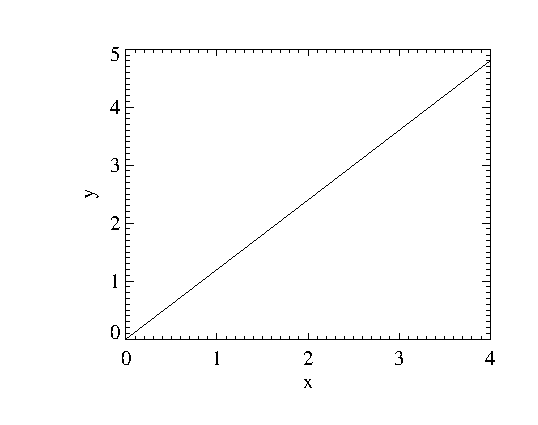
\includegraphics[width=3.75in]{simple.eps}
  \end{center}
  \caption{The caption of the figure.}
\label{fig:fig00}
\end{figure}%
\lipsum[5]

\subsection{Figure with psfrag Replacement}

\lipsum[8].  Figure~\ref{fig:fig01} illustrates the use
of the psfrag package to place \LaTeX\ math in a graphic.%
\begin{figure}[tb]
  \psfrag{x}{$x$}
  \psfrag{y}{$y$}
  \begin{center}
   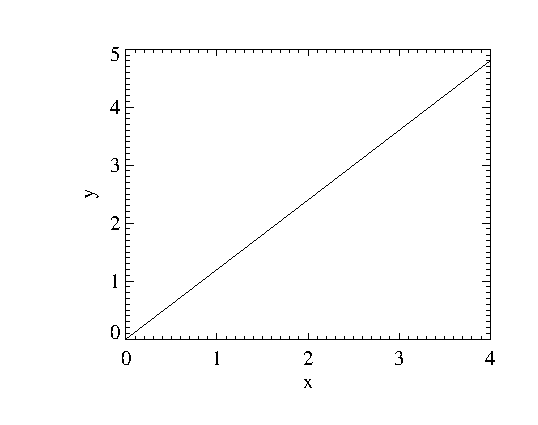
\includegraphics[width=3.75in]{simple.eps}
  \end{center}
  \caption[A figure caption which is extra long.]{A figure caption
    which is extra long. This long caption not only demonstratees that
    the required spacing in the list of figures is correct, but also
    the general practice of making the list of figures (or tables)
    entry the first sentence of the caption.}
\label{fig:fig01}
\end{figure}
\lipsum[1]. The filler content is followed by a second figure,
Figure~\ref{fig:fig02}.  %
\begin{figure}[tb]
  \psfrag{x}{$\hat{x}/L$}
  \psfrag{y}{$y$}
  \begin{center}
   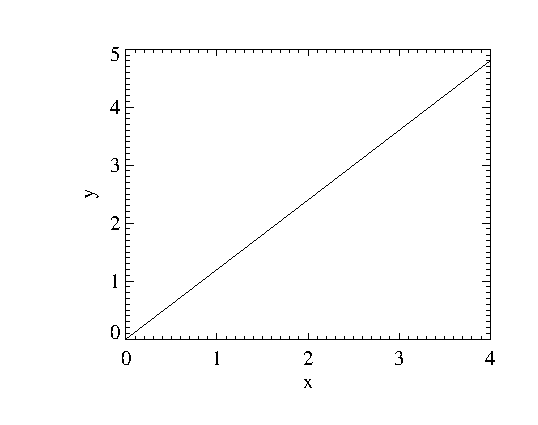
\includegraphics[width=3.75in]{simple.eps}
  \end{center}
  \caption{The figure caption made extra long so that the
    required spacing in the list of figures is evident.}
\label{fig:fig02}
\end{figure}
\lipsum[9]
\section{Section with Sample Tables}

\subsection{Simple Table}

Finally the tables, Table~\ref{tbl:tbl01} illustrates the syntax of a
basic table. %
\begin{table}[tb]
  \caption{The capitalization of the table should match that of figures.}
  \label{tbl:tbl01}
  \begin{center}
  \begin{tabular}{c l l}
  \hline
  Example & Time & Cost \\
  \hline
  1 & 12.5 & \$1,000 \\
  2 & 24 & \$2,000 \\
  \hline
  \end{tabular}
  \end{center}
\end{table}

\subsection{Three-Part Table}

Table~\ref{tbl:tbl02}, which illustrates the syntax of a three-part
table which includes table notes in addition to a caption and table
body.
\begin{table}[tb]
\begin{threeparttable}
  \caption{The caption of the three-part table.}
  \label{tbl:tbl02}
  \begin{center}
\begin{tabular*}{\textwidth}{c l l} % or {tabular}
  \hline
  Example & Time\tnote{1} & Cost \\
  \hline
  1 & 12.5 & \$1,000 \\
  2 & 24 & \$2,000 \\
  \hline
\end{tabular*}
\begin{tablenotes}
  \item [1] The first note.
\end{tablenotes}
  \end{center}
\end{threeparttable}
\end{table}
\lipsum[11-12]


\section{Section with \texttt{natbib} Citations}

This had been discussed previously by \citep{bullwinkle:1990} and
\citet{bullwinkle:1991}. \lipsum[10-11]


\section{Section with \texttt{nomencl} Entries}

 This is my simple equation to illustrate the use of the nomencl
 package for automatic generation of a list of symbols.
\begin{equation}
\delta_i = \sqrt{t/\mathrm{Pe}}
\end{equation}
where $\delta$ is the layer
thickness %
\nomenclature[at]{$t$}{time}%
\nomenclature[gd]{$\delta$}{layer thickness}%
\nomenclature[si]{$i$}{inlet}%
as defined previously. \lipsum[13]
\endinput
%%
%% End of file `chapall.tex'.


\end{ThesisBody}
%    \end{macrocode}
%
% \subsubsection{Appendix}
%
%    \begin{macrocode}
 % ... appendix - specify number of appendix chapters ...

\begin{ThesisAppendix}{two}
\ThesisAppendixChapter{One}%%
%% This is file `chapbib.tex',
%% generated with the docstrip utility.
%%
%% The original source files were:
%%
%% ths.dtx  (with options: `chapmin,addbib')
%% 
%% IMPORTANT NOTICE:
%% 
%% For the copyright see the source file.
%% 
%% Any modified versions of this file must be renamed
%% with new filenames distinct from chapbib.tex.
%% 
%% For distribution of the original source see the terms
%% for copying and modification in the file ths.dtx.
%% 
%% This generated file may be distributed as long as the
%% original source files, as listed above, are part of the
%% same distribution. (The sources need not necessarily be
%% in the same archive or directory.)


 %% ... sample chapter ...

\lipsum[5]

\section{Introduction}
\lipsum[6-8]


\section{Section with \texttt{natbib} Citations}

This had been discussed previously by \citep{bullwinkle:1990} and
\citet{bullwinkle:1991}. \lipsum[10-11]

\endinput
%%
%% End of file `chapbib.tex'.

\ThesisAppendixChapter{Two}%%
%% This is file `chapbib.tex',
%% generated with the docstrip utility.
%%
%% The original source files were:
%%
%% ths.dtx  (with options: `chapmin,addbib')
%% 
%% IMPORTANT NOTICE:
%% 
%% For the copyright see the source file.
%% 
%% Any modified versions of this file must be renamed
%% with new filenames distinct from chapbib.tex.
%% 
%% For distribution of the original source see the terms
%% for copying and modification in the file ths.dtx.
%% 
%% This generated file may be distributed as long as the
%% original source files, as listed above, are part of the
%% same distribution. (The sources need not necessarily be
%% in the same archive or directory.)


 %% ... sample chapter ...

\lipsum[5]

\section{Introduction}
\lipsum[6-8]


\section{Section with \texttt{natbib} Citations}

This had been discussed previously by \citep{bullwinkle:1990} and
\citet{bullwinkle:1991}. \lipsum[10-11]

\endinput
%%
%% End of file `chapbib.tex'.

\end{ThesisAppendix}

%    \end{macrocode}
%
% \subsubsection{Back Matter - References and Vita}
%
%    \begin{macrocode}
 % ... references - comma separated list of bib files ...

\newpage\bibliographystyle{plainnat}
\bibliography{add.bib}

 % ... vita ...

\begin{Vita}
\lipsum[3]
\end{Vita}

\end{document}
%</rpc>
%    \end{macrocode}
%
% \section{\LaTeX\ Template for Publication Thesis Option}
%
% \subsection{Using the Template}
%
% The steps in using the Publication Thesis Option template are the
% following
% \begin{enumerate}
% \item In each \verb|ppr.tex| file, change the class options
%   in the documentclass command to 
%   \verb|\documentclass[times,thesis]{journal}| where \emph{journal}
%   is the name of the journal the paper formatted for.  Once the class
%   options have been changed, re-make the file.  This should produce a 
%   postscript file with margins and pagination obeying the thesis
%   requirements.
% \item In each \verb|ppr.tex| file, add the following command
%   \verb|\setcounter{page}{x}| immediately following the 
%   \verb|\begin{document}| command, where \emph{x} is the starting page
%   number for the corresponding paper.  Now re-make each of the 
%   \verb|ppr.tex| files.  The result should be a thesis body with each of
%   the papers consituting it numbered consecutively.
% \item Edit the thesis.tex template by entering the correct paper names
%   and so on.  Compile the thesis template with the make command. Make
%   sure the pagination for the table of contents entries with the 
%   thesis body are correct.  Note that in the template, the setcounter
%   command will need to be issued with the correct page number corresponding
%   to each individual paper.
% \item Add (or uncomment) the \verb|\nofiles| command to the template
%   immediately preceding the \verb|\begin{document}| command.  This
%   command prevents \LaTeX\ from writing any changes to the 
%   \verb|.toc,.lof,.lot| files.  
% \item Add the entire contents from each \verb|ppr.lof| and \verb|ppr.lot|
%   to the corresponding template \verb|.lof| or \verb|.lot| file, at the 
%   appropriate place in these files.  Then recompile the 
%   template and be sure the the list of figures and list of tables entries
%   generated are correct.
% \item Now, go back to the individual \verb|ppr.tex| files and add
%   the \verb|\tableofcontents| command to each and re-make them.  Now
%   copy the contents of each of these individual \verb|.toc| files
%   to the \verb|.toc| file of the thesis template. Re-make the thesis.
% \item Print out the \verb|ppr.ps| files and the \verb|thesis.ps| files, 
%   put them in order and you have a complete thesis.
% \end{enumerate}
%
% \subsection{Additional Notes and Hints}
%
% \begin{itemize}
% \item If the bibliography in an individual entry needs to be edited
%   directly, edit the \verb|ppr.bbl| file but make sure not to re-run
%   the bibtex command because otherwise the changes will be overwritten.
% \item The \verb|nofiles| command cannot be used in the individual
%   \verb|ppr.tex| files since otherwise the nomenclature is not generated.
% \item In the thesis list of tables and list of illustrations, only an
%   abbreviated caption should appear.  This can be accomplished by editing
%   the \verb|.lof| and \verb|.lot| files.  Preferably, however, it can be
%   accomplished by using the following form of the caption command:
%   \verb|\caption[lst_entry]{heading}| where \verb|lst_entry| is the
%   abbreviated entry which is to appear in the list of figures or tables.
%   This can be the first sentence of the extended caption or an 
%   even more abbreviated version.
% \item The individual entries in the list of figures and tables for 
%   each paper must be set off by the following 
%   \verb|\noindent\mbox{PAPER 1\hfill}\nopagebreak|.  This should be 
%   added to the \verb|.lot| and \verb|.lof| files.
% \item The block of entries the \verb|.toc| must also be set off by a
%   command identical to the above.  In addition, this should be
%   preceded by \verb|\addvspace{\baselineskip}|.
% \item The list of figures and tables must also have single-spaced 
%   entries with doublespacing between the entries.  A way to 
%   accomplish this is to put the \verb|\singlespacing| command as the
%   second line of the \verb|.lot| and \verb|.lof| files and add,
%   immediately in front of each contentsline command, the following:
%   \verb|\addvspace{\baselineskip}|.  This same command will need to
%   be added in front of each of the above Paper x commands so that 
%   there is a blank line between the last entry of one paper and 
%   the line that says \verb|Paper x+1|.
% \item The entries in the table of contents must also be single spaced
%   for each entry and double-spaced between.  However, it is easier to
%   just let the table of contents be double-spaced and then put an
%   individual table of contents inside a singlespacing environment, if
%   it requires more than one line.
% \end{itemize}
%
% \subsection{Thesis Template}
%
% \subsubsection{Preamble}
%
% The preamble is ended by the \verb|\begin{document}| command.
% 
%    \begin{macrocode}
%<*pto>
 % -*- mode: LaTeX -*-
 % ... preamble ...
\documentclass[times,12pt,titlepage]{mstthesis}
\doublespacing

\usepackage{fancyhdr}
\pagestyle{fancy}
\lhead{}\chead{}\rhead{\thepage}
\lfoot{}\cfoot{}\rfoot{}
\renewcommand{\headrulewidth}{0pt}
\renewcommand{\footrulewidth}{0pt}

\usepackage[nopar]{lipsum}

 % ... uncomment after editing toc, lof, lot ...

 %\nofiles

 % ... end preamble ...

\begin{document}

%    \end{macrocode}
%
% \subsubsection{Title Page}
%
%    \begin{macrocode}

 % ... specify: ms | phd ...

\begin{ThesisTitlePage}{ms}

\author{\MakeUppercase{I. M. Author}}

\thesistitle{\MakeUppercase{The Title of My Work}}

\department{Mechanical Engineering}

 % ... thesis committee ...

\ThesisAdviser{Galileo}

 % If you have a co-advisor, enter the name in the 
 % curly braces below and uncomment.  
 % Otherwise, leave commented out.
 %\cothadviser{} % If you have 2 thesis advisers

\memberone{Newton}        
\membertwo{Copernicus}        
\memberthree{Laplace}
\memberfour{Fourier}
\memberfive{}

 % ... Graduation date.  NOT your submission date! ...
\graddate{1685}       

\end{ThesisTitlePage}
%    \end{macrocode}
%
% \subsubsection{Copyright, Abstract and Acknowledgments}
%
%    \begin{macrocode}

 % ... copyright page - true|false ...

\copyrightyear{1684}
\ThesisCopyrightPage{false}

 % ... front matter - publication option - ms|phd...

\begin{ThesisPublicationOption}{phd}
  This thesis (or dissertation) has been prepared in the style
  utilized by the Journal of Everything Important.  Pages 1-17 will be
  submitted for publication in that journal.  Appendices A, B and C
  have been added for purposes normal to thesis/dissertation writing.
  This thesis or dissertation has been prepared in the form of three
  papers.
\end{ThesisPublicationOption}

 % ... front matter - thesis abstract ...

\begin{ThesisAbstract}
\lipsum[1]
\end{ThesisAbstract}

 % ... front matter - acknowledgements ...

\begin{ThesisAcknowledgment}
\lipsum[2]
\end{ThesisAcknowledgment}

%    \end{macrocode}
%
% \subsubsection{Contents, Illustrations, Tables and Symbols}
%
%    \begin{macrocode}
 % ... toc, lof, and lot (list of symbols in respective papers) ...
\begin{ThesisFrontMatter}
\tableofcontents
\listoffigures
\listoftables
\end{ThesisFrontMatter}

%    \end{macrocode}
%
% \subsubsection{Thesis Body}
%
%    \begin{macrocode}
 % ... introduction chapter ...

\begin{ThesisBody}

\begin{ThesisOnlyChapters}
\ThesisBodyChapter{Introduction}%%
%% This is file `chapmin.tex',
%% generated with the docstrip utility.
%%
%% The original source files were:
%%
%% ths.dtx  (with options: `chapmin')
%% 
%% IMPORTANT NOTICE:
%% 
%% For the copyright see the source file.
%% 
%% Any modified versions of this file must be renamed
%% with new filenames distinct from chapmin.tex.
%% 
%% For distribution of the original source see the terms
%% for copying and modification in the file ths.dtx.
%% 
%% This generated file may be distributed as long as the
%% original source files, as listed above, are part of the
%% same distribution. (The sources need not necessarily be
%% in the same archive or directory.)


 %% ... sample chapter ...

\lipsum[5]

\section{Introduction}
\lipsum[6-8]

\endinput
%%
%% End of file `chapmin.tex'.

\ThesisBodyChapter{Literature Review}%%
%% This is file `chapmin.tex',
%% generated with the docstrip utility.
%%
%% The original source files were:
%%
%% ths.dtx  (with options: `chapmin')
%% 
%% IMPORTANT NOTICE:
%% 
%% For the copyright see the source file.
%% 
%% Any modified versions of this file must be renamed
%% with new filenames distinct from chapmin.tex.
%% 
%% For distribution of the original source see the terms
%% for copying and modification in the file ths.dtx.
%% 
%% This generated file may be distributed as long as the
%% original source files, as listed above, are part of the
%% same distribution. (The sources need not necessarily be
%% in the same archive or directory.)


 %% ... sample chapter ...

\lipsum[5]

\section{Introduction}
\lipsum[6-8]

\endinput
%%
%% End of file `chapmin.tex'.

\end{ThesisOnlyChapters}

 % ... thesis publications ...

\begin{ThesisPublications}
\PaperManuscript{I}{MY FIRST PAPER TITLE}
\PaperManuscript{II}{MY SECOND PAPER TITLE}
\PaperManuscript{III}{MY THIRD PAPER TITLE}
\end{ThesisPublications}

 % ... conclusions chapter ...

\begin{ThesisOnlyChapters}
\ThesisBodyChapter{My Summary and Conclusions}%%
%% This is file `chapmin.tex',
%% generated with the docstrip utility.
%%
%% The original source files were:
%%
%% ths.dtx  (with options: `chapmin')
%% 
%% IMPORTANT NOTICE:
%% 
%% For the copyright see the source file.
%% 
%% Any modified versions of this file must be renamed
%% with new filenames distinct from chapmin.tex.
%% 
%% For distribution of the original source see the terms
%% for copying and modification in the file ths.dtx.
%% 
%% This generated file may be distributed as long as the
%% original source files, as listed above, are part of the
%% same distribution. (The sources need not necessarily be
%% in the same archive or directory.)


 %% ... sample chapter ...

\lipsum[5]

\section{Introduction}
\lipsum[6-8]

\endinput
%%
%% End of file `chapmin.tex'.

\end{ThesisOnlyChapters}

\end{ThesisBody}

%    \end{macrocode}
%
% \subsubsection{Appendix}
%
%    \begin{macrocode}
 % ... appendix - specify number of appendix chapters ...

\begin{ThesisAppendix}{two}
\ThesisAppendixChapter{One}%%
%% This is file `chapbib.tex',
%% generated with the docstrip utility.
%%
%% The original source files were:
%%
%% ths.dtx  (with options: `chapmin,addbib')
%% 
%% IMPORTANT NOTICE:
%% 
%% For the copyright see the source file.
%% 
%% Any modified versions of this file must be renamed
%% with new filenames distinct from chapbib.tex.
%% 
%% For distribution of the original source see the terms
%% for copying and modification in the file ths.dtx.
%% 
%% This generated file may be distributed as long as the
%% original source files, as listed above, are part of the
%% same distribution. (The sources need not necessarily be
%% in the same archive or directory.)


 %% ... sample chapter ...

\lipsum[5]

\section{Introduction}
\lipsum[6-8]


\section{Section with \texttt{natbib} Citations}

This had been discussed previously by \citep{bullwinkle:1990} and
\citet{bullwinkle:1991}. \lipsum[10-11]

\endinput
%%
%% End of file `chapbib.tex'.

\ThesisAppendixChapter{Two}%%
%% This is file `chapbib.tex',
%% generated with the docstrip utility.
%%
%% The original source files were:
%%
%% ths.dtx  (with options: `chapmin,addbib')
%% 
%% IMPORTANT NOTICE:
%% 
%% For the copyright see the source file.
%% 
%% Any modified versions of this file must be renamed
%% with new filenames distinct from chapbib.tex.
%% 
%% For distribution of the original source see the terms
%% for copying and modification in the file ths.dtx.
%% 
%% This generated file may be distributed as long as the
%% original source files, as listed above, are part of the
%% same distribution. (The sources need not necessarily be
%% in the same archive or directory.)


 %% ... sample chapter ...

\lipsum[5]

\section{Introduction}
\lipsum[6-8]


\section{Section with \texttt{natbib} Citations}

This had been discussed previously by \citep{bullwinkle:1990} and
\citet{bullwinkle:1991}. \lipsum[10-11]

\endinput
%%
%% End of file `chapbib.tex'.

\end{ThesisAppendix}

%    \end{macrocode}
%
% \subsubsection{Back Matter - References and Vita}
%
%    \begin{macrocode}
 % ... references - comma separated list of bib files ...

\newpage\bibliographystyle{plainnat}
\bibliography{add.bib}

 % ... vita ...

\begin{Vita}
\lipsum[3]
\end{Vita}

 % ... end document ...

\end{document}
%</pto>
%    \end{macrocode}
%
% \section{\LaTeX\ Templates for Generic Chapter Content}
%
% \subsection{Minimal (text-only) Chapter Template}
%
%    \begin{macrocode}
%<*chapmin>

 %% ... sample chapter ...

\lipsum[5]

\section{Introduction}
\lipsum[6-8]

%</chapmin>
%    \end{macrocode}
%
% \subsection{Section with Figures}
%
%    \begin{macrocode}
%<*addfig>
\section{Section with Figures and Heading Which is Really Long So 
That It Produces a Two-Line Toc Entry}
\lipsum[9]

\subsection{Simple Figure with Label}

Add a simple figure, Figure~\ref{fig:fig00}, to illustrate
an entry in the list of figures. %
\begin{figure}[tb]
  \begin{center}
   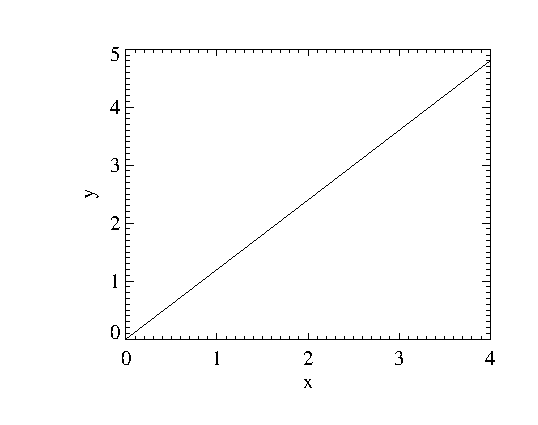
\includegraphics[width=3.75in]{simple.eps}
  \end{center}
  \caption{The caption of the figure.}
\label{fig:fig00}
\end{figure}%
\lipsum[5]

\subsection{Figure with psfrag Replacement}

\lipsum[8].  Figure~\ref{fig:fig01} illustrates the use
of the psfrag package to place \LaTeX\ math in a graphic.%
\begin{figure}[tb]
  \psfrag{x}{$x$}
  \psfrag{y}{$y$}
  \begin{center}
   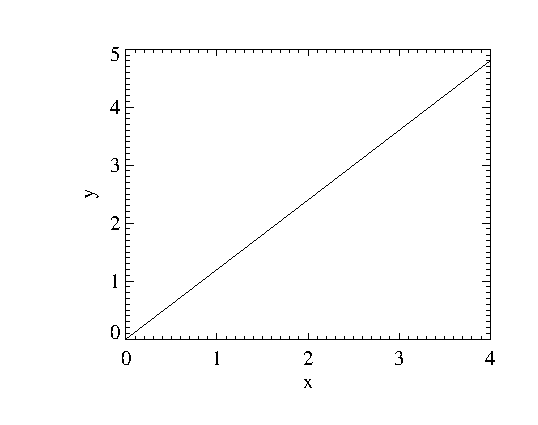
\includegraphics[width=3.75in]{simple.eps}
  \end{center}
  \caption[A figure caption which is extra long.]{A figure caption
    which is extra long. This long caption not only demonstratees that
    the required spacing in the list of figures is correct, but also
    the general practice of making the list of figures (or tables)
    entry the first sentence of the caption.}
\label{fig:fig01}
\end{figure}
\lipsum[1]. The filler content is followed by a second figure,
Figure~\ref{fig:fig02}.  %
\begin{figure}[tb]
  \psfrag{x}{$\hat{x}/L$}
  \psfrag{y}{$y$}
  \begin{center}
   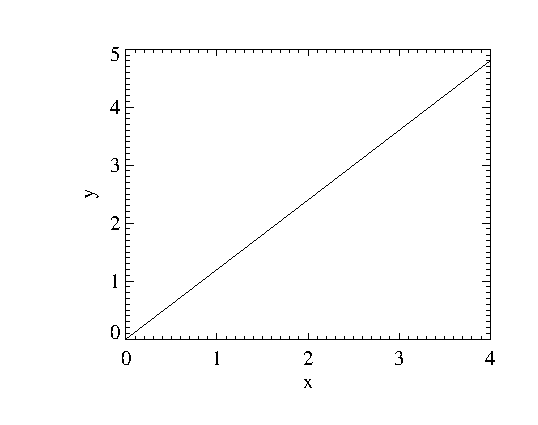
\includegraphics[width=3.75in]{simple.eps}
  \end{center}
  \caption{The figure caption made extra long so that the
    required spacing in the list of figures is evident.}
\label{fig:fig02}
\end{figure}
\lipsum[9]
%</addfig>
%    \end{macrocode}
%
% \subsection{Section with Tables}
%
%    \begin{macrocode}
%<*addtbl>
\section{Section with Sample Tables}

\subsection{Simple Table}

Finally the tables, Table~\ref{tbl:tbl01} illustrates the syntax of a
basic table. %
\begin{table}[tb]
  \caption{The capitalization of the table should match that of figures.}
  \label{tbl:tbl01}
  \begin{center}
  \begin{tabular}{c l l}
  \hline
  Example & Time & Cost \\
  \hline
  1 & 12.5 & \$1,000 \\
  2 & 24 & \$2,000 \\
  \hline
  \end{tabular}
  \end{center}
\end{table}

\subsection{Three-Part Table}

Table~\ref{tbl:tbl02}, which illustrates the syntax of a three-part
table which includes table notes in addition to a caption and table
body.
\begin{table}[tb]
\begin{threeparttable}
  \caption{The caption of the three-part table.}
  \label{tbl:tbl02}
  \begin{center}
\begin{tabular*}{\textwidth}{c l l} % or {tabular}
  \hline
  Example & Time\tnote{1} & Cost \\
  \hline
  1 & 12.5 & \$1,000 \\
  2 & 24 & \$2,000 \\
  \hline
\end{tabular*}
\begin{tablenotes}
  \item [1] The first note.
\end{tablenotes}
  \end{center}
\end{threeparttable}
\end{table}
\lipsum[11-12]

%</addtbl>
%    \end{macrocode}
%
% \subsection{Section with \texttt{natbib} Citations}
%
%    \begin{macrocode}
%<*addbib>

\section{Section with \texttt{natbib} Citations}

This had been discussed previously by \citep{bullwinkle:1990} and
\citet{bullwinkle:1991}. \lipsum[10-11]

%</addbib>
%    \end{macrocode}
%
% \subsection{Section with \texttt{nomencl} Entries} 
%
%    \begin{macrocode}
%<*addglo>

\section{Section with \texttt{nomencl} Entries} 

 This is my simple equation to illustrate the use of the nomencl
 package for automatic generation of a list of symbols.
\begin{equation}
\delta_i = \sqrt{t/\mathrm{Pe}}
\end{equation}
where $\delta$ is the layer
thickness %
\nomenclature[at]{$t$}{time}%
\nomenclature[gd]{$\delta$}{layer thickness}%
\nomenclature[si]{$i$}{inlet}%
as defined previously. \lipsum[13]
%</addglo>
%    \end{macrocode}
%
\endinput       

% **** **** **** **** **** **** **** **** **** **** ****
% ... Version Control Log ...
%
%  $Id: ths.dtx,v 6.4 2015/02/17 19:12:42 khoman Exp $
%
% $Log: ths.dtx,v $
% Revision 6.4  2015/02/17 19:12:42  khoman
% Replaced occurrences of <ps> with space+%, which removes need for the
% associated sed replacement.
%
% Revision 6.3  2015/01/28 18:27:54  khoman
% Removed rcsinfo commands from template content.
%
% Revision 6.2  2014/10/21 19:27:56  khoman
% Revised documentation in preparation for campus-wide distribution.
%
% Revision 6.1  2014/10/21 18:05:09  khoman
% Initial version for distribution through OGS.
%
% Revision 5.2  2014/09/17 14:20:34  khoman
% Revised the publication thesis option template to reflect the new
% environment ThesisOnlyChapters.
%
% Revision 5.1  2014/08/13 18:01:14  khoman
% Completed OGS-indicated revisions for rpc thesis and almost all of the
% revisions for the pto thesis.
%
% Revision 4.3  2014/08/12 22:07:52  khoman
% Edits through partial update of toc formatting.
%
% Revision 4.2  2014/08/12 15:27:17  khoman
% Title page now conforms to requested standard.
%
% Revision 4.1  2014/08/12 14:58:36  khoman
% Revisions up to and including initial development of campus-standard
% class and template file.
%
% Revision 3.2  2012/07/26 16:13:11  khoman
% Edited the templates so that now the ThesisBodyChapter and
% ThesisAppendixChapter commands are used.  The chapter command was then
% also removed from the chapmin chunk.
%
% Revision 3.1  2012/07/25 21:39:35  khoman
% Major revision of the template file prompted by the work of Ben
% Payne's PhD use of my class file and template.  The primary change in
% the present version is the movement of the lipsum package and a
% re-organization of the sample chapter content so that it is entirely
% generic to both the pto and the rpc thesis templates.  In addition,
% the fig, tbl, bib citation and glo entry samples were moved into
% separate chunks, which themselves constitute a separate section.  A
% minimal chapter can then have fig, tbl, bib and/or glo content added
% to it by appending these chunks.  The basic content in the sample
% chapters is largely unchanged from the previous v2 of this file.
%
% Revision 2.8  2012/02/23 04:46:38  khoman
% Added a second appendix to the rpctemplate and added the same
% two-chapter appendix to the ptotemplate.  This was added to
% demonstrate the behavior with multiple appendix chapters.  The
% resulting behavior is correct.
%
% Revision 2.7  2011/11/04 17:13:05  khoman
% Removed thispagestyle{empty} command after first invocation of the
% chapter command in thesis body.
%
% Revision 2.6  2011/11/03 14:24:50  khoman
% Changes made based on suggestions by Phil Thiem.
%
% Revision 2.5  2011/11/01 15:08:39  khoman
% Capitalized first letter of each word in section and subsection headings.
%
% Revision 2.4  2011/10/27 15:29:44  khoman
% Added hints from James Tinsley regarding widow and orphan lines.
%
% Revision 2.3  2011/10/26 16:14:44  khoman
% Changed the default class option to times font which invokes the
% publically-available times roman fonts.
%
% Revision 2.2  2011/10/26 14:30:42  khoman
% Minor changes - made computer modern the default font and added a long
% section heading to show the class properly handles this both in the
% text and in the table of contents.
%
% Revision 2.1  2011/10/25 17:26:24  khoman
% The two templates, report class and publication thesis option, work
% correctly with the mstthesis.cls file produced by v2 theses.dtx.  The
% template files are very clean now and use environments to hide all of
% the lower level formatting specifications and details.
%
% Revision 1.5  2011/10/20 22:11:52  khoman
% Revisions to report class template corresponding to the issues noted
% by first round of thesis check for James Tinsley MS.
%
% Revision 1.4  2011/10/11 14:34:28  khoman
% Commented out the explicit toc commands for the chapters.
%
% Revision 1.3  2011/07/14 18:13:16  khoman
% Completed revision as part of developing the report class thesis
% template.  The template works correctly with the current version of
% the mstthesis.cls file.
%
% Revision 1.2  2008/01/23 19:21:56  khoman
% Added the how to use content as well as hints and tips for the
% publication thesis option template.  The template should be bug
% free. However, some additional refinement could certainly be done.
%
% Revision 1.1  2008/01/23 15:27:11  khoman
% Initial revision
%
% Revision 2.16  2004/10/28 16:41:27  khoman
% Added citet command so that both the citep and citet commands are
% illustrated.
%
% Revision 2.15  2004/04/13 18:50:48  khoman
% Added firstauthor command for use with submit option of asme class.
%
% Revision 2.14  2004/02/23 20:48:33  khoman
% Updated to reflect changes in the journal class files.
%
% Revision 2.13  2004/02/20 15:33:55  khoman
% Corrected poor grammar in nompreamble.
%
% Revision 2.12  2004/02/20 15:29:21  khoman
% Removed the redefinition of the refname.
%
% Revision 2.11  2004/02/20 15:26:30  khoman
% Removed specification of the bibliography style file as it has been
% moved to the class file.
%
% Revision 2.10  2004/01/29 19:30:32  khoman
% Moved strings.bib to first position in bibliography command and
% updated name of the dtx file.
%
% Revision 2.9  2003/07/11 13:37:08  khoman
% Corrected specification of the LaTeX mode.
%
% Revision 2.8  2003/07/11 13:32:28  khoman
% Added sed replacements for the percent sign within the macrocode, as
% is done with the noweb templates.
%
% Revision 2.7  2003/07/08 21:27:50  khoman
% Changed bib files to all of the bibs.
%
% Revision 2.6  2003/06/13 16:26:53  khoman
% Changed "Printed" in date to "LaTeX'd on".
%
% Revision 2.5  2002/12/05 10:09:49  khoman
% Moved the nomenclature section from immediately after the abstract to
% immediately after the acknowledgments.  This arrangement is consistent
% with current ASME practice.
%
% Revision 2.4  2002/11/21 14:34:16  khoman
% Removed input command from the abstract.
%
% Revision 2.3  2002/11/21 14:25:09  khoman
% Slight revision of the sectioning levels.
%
% Revision 2.2  2002/11/21 14:16:55  khoman
% Moved the version control log to after the endinput command.
%
% Revision 2.1  2002/11/21 14:14:45  khoman
% Added examples of addchange and delchange environments.  Also added
% commands immediately following maketitle which take care of the line
% spacing and the headings.
%
% Revision 1.23  2002/10/25 11:18:27  khoman
% Added additional commands for formatting draft class option.
%
% Revision 1.22  2002/10/24 15:25:06  khoman
% Added rcsinfo version and date to header.
%
% Revision 1.21  2001/11/07 15:00:58  khoman
% Added an explanatory note to the nomenclature example outlining the
% use of the prefix characters to generate appropriate alphabetizing of
% the symbols.
%
% Revision 1.20  2001/09/19 17:51:27  khoman
% Changed my author address to UMR.
%
% Revision 1.19  2001/04/24 15:59:29  khoman
% Added nompreamble command to add note at beginning of nomenclature
% list prior to any entries.
%
% Revision 1.18  2001/03/28 21:58:56  khoman
% Removed academic title from author block.
%
% Revision 1.17  2001/03/28 21:00:55  khoman
% Removed the rcsinfo date from the title thanks since it would be
% misread to mean the submission date when it actually is the date of
% the last rcs check-in.
%
% Revision 1.16  2001/01/31 21:29:20  khoman
% Updated the author info to reflect the revisions to the journal classes.
%
% Revision 1.15  2001/01/31 20:58:40  khoman
% Moved the location of the ifthenelse statement to just following the
% maketitle command so that the title and author information are not
% doublespaced.
%
% Revision 1.14  2001/01/05 17:59:49  khoman
% Formatted the revision log.
%
% Revision 1.13  2000/12/31 08:14:14  khoman
% Uncommented the input of the mydefs.tex file.  The file was loaded
% through a symbolic link.
%
% Revision 1.12  2000/12/31 07:57:58  khoman
% Changed references to hvacr.cls to ijhvacr.cls, reflecting the changes
% in the journals.dtx file.
%
% Revision 1.11  2000/12/29 17:03:32  khoman
% Removed the local command definitions and replaced them with an input 
% of mydefs.tex.
%
% Revision 1.10  2000/12/29 07:06:14  khoman
% Added an eps file and psfrag commands as the figure example.  Changed
% the content and format of the title thanks.  Formatted the revision
% log.
%
% Revision 1.9  2000/12/29 06:11:03  khoman
% Removed rcs head and tail comment blocks.
%
% Revision 1.8  2000/12/19 16:15:24  khoman
% Added eqn, fig and tbl commands as first used in the nhtc01 paper.
%
% Revision 1.7  2000/12/18 15:49:50  khoman
% Commented out the asme conference proceedings commands and put the rcs
% id and log commands behind comments characters.
%
% Revision 1.6  2000/12/17 02:23:21  khoman
% Added refname change to just before the bibliography command since
% placing it in the cls file or anywhere before the begin document
% seems to get overwritten.
%
% Revision 1.5  2000/12/16 07:59:24  khoman
% Added asme proceedings commands.
%
% Revision 1.4  2000/12/15 17:56:57  khoman
% Added comment to template indicating the available options for each of
% the defined classes.
%
% Revision 1.3  2000/10/04 20:00:17  khoman
% Added an example bibliographic entry using the single entry
% template.bib file.  Also changed the bibliography style to plain from
% asmeauthordate.
%
% Revision 1.2  2000/10/03 13:47:21  khoman
% Removed the invocation of the noweb mode for emacs.
%
% Revision 1.1  2000/10/03 13:19:17  khoman
% Initial revision
%
% **** **** **** **** **** **** **** **** **** **** ****










